\graphicspath{{Images/control/}}

\chapter{Tracking Control of a Miniature 2-DOF Manipulator with Hydrogel Actuators}
\label{chap:control}
Due to the nature of the complex spatiotemporal dynamics of stimuli-responsive soft materials, closed-loop control of hydrogel-actuated mechanisms has remained a challenge. This paper demonstrates, for the first time, closed-loop trajectory tracking control in real-time of a millimeter-scale, two degree-of-freedom manipulator via \emph{independently-controllable}, temperature-responsive hydrogel actuators. A linear state-space model of the manipulator is developed from input-output measurement data, enabling the straightforward application of control techniques to the system. The Normalized Mean Absolute Error~(NMAE) between the modeled and measured displacement of the manipulator's tip is below 10\%. We propose an Observer-based controller and a robust $H_{\infty}$-optimal controller and evaluate their 
% stability and convergence properties. The controllers' 
performance in a trajectory tracking output-feedback framework, compared with and without sinusoidal disturbances and noise. We demonstrate in simulation that the $H_\infty$-optimal controller, which is computed using Linear Matrix Inequality (LMI) methods, tracks an elliptical trajectory more accurately than the Observer controller and is more robust to disturbances and noise. We also show experimentally that the $H_\infty$-optimal controller can be used to track different trajectories with an NMAE below 15$\%$, even when the manipulator is subject to a 3\,g load, 12.5 times an actuator's weight. Finally, a payload transport scenario is presented as an exemplar application; we demonstrate that an array of four manipulators is capable of moving a payload horizontally by applying the proposed $H_\infty$-optimal trajectory-tracking controller to each manipulator in a decoupled manner.
\section{Background}
Soft actuators, composed of deformable matter such as fluids, gels, elastomers, and shape memory alloys (SMAs)~\cite{Majidi2014}, are lightweight and noiseless, in contrast to pneumatic systems with pumps and motors. Stimuli-responsive materials have potential applications in micro-manipulation, sensing, optics~\cite{Mantha2019,Qin2019}, and biomedical applications~\cite{Guiseppi-Elie2010}. Hydrogels in particular have the ability to absorb and release water, undergoing reversible volumetric changes that facilitates their use as soft actuators~\cite{Mishra2020}. A variety of hydrogel formulations exist, enabling these materials to change state under different external physical or chemical stimuli~\cite{Peng2018,He2012}. For example, poly(N-isopropylacrylamide), or PNIPAAM, is a commonly used temperature-responsive hydrogel that contracts when heated.

\begin{figure}[h]
\centering
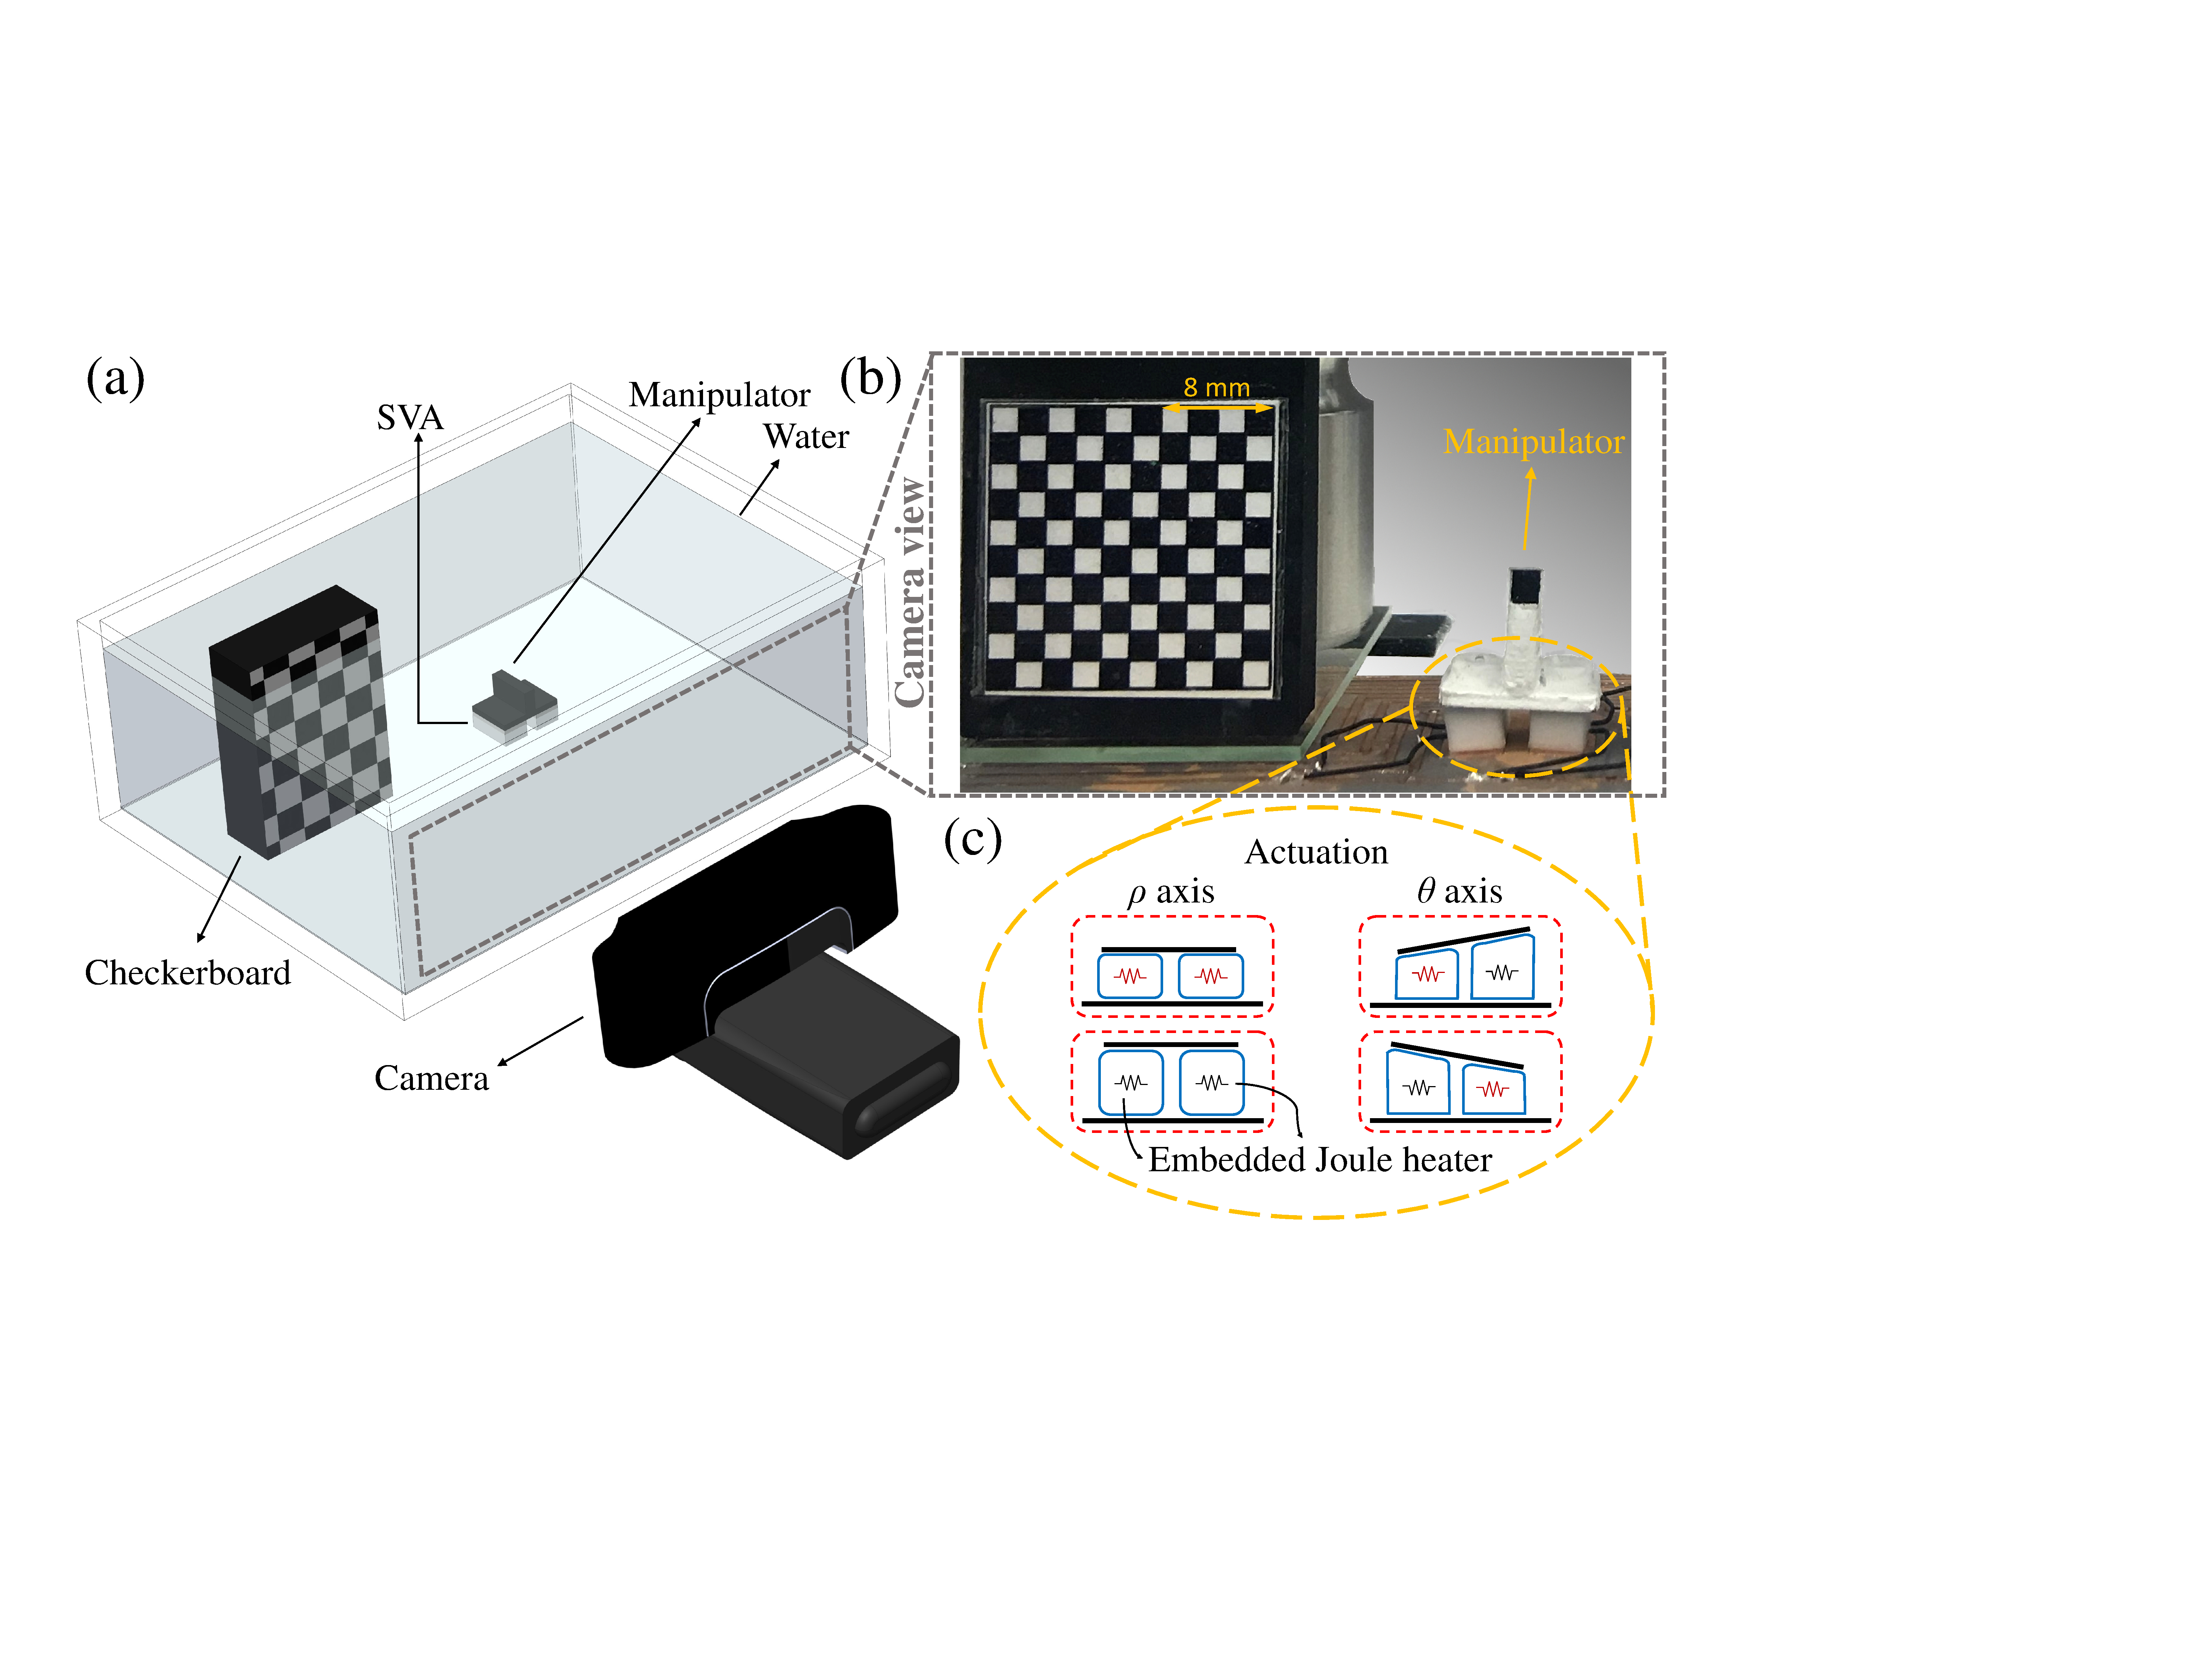
\includegraphics[width=\textwidth]{ConceptDesign6_O.pdf}
    \caption[Experimental setup for tracking control of a 2-DOF manipulator]{Experimental setup for tracking control of a 2-DOF manipulator with embedded hydrogel Soft Voxel Actuators (SVAs)~\cite{Doroudchi2020}. (a) Illustration of a manipulator in a water-filled tank with a camera for vision-based feedback of the manipulator tip. (b) Camera view of the setup, including a fabricated 
    manipulator prototype and checkerboard for camera calibration. (c) Illustration of SVA deformation in various activation states (red = on; black = off).}
    \vspace{-0.75cm}
    \label{fig:setup}
\end{figure}

Hydrogel-based active mechanisms using morphing or bending beams and sheets have been utilized for sensing, smart micro-fluidic valves, optical lensing, and micro-scale swimming and walking~\cite{Ionov2014}. More complicated tasks, such as picking and placing objects with open-loop control methods, have also been demonstrated~\cite{Wang2015b}. Due to the nature of the stimuli, closed-loop control of hydrogel actuators has remained a challenge. Light sources such as lasers~\cite{Luo2015}, for instance, require sophisticated and bulky equipment to produce motion. The methods used in~\cite{Kim2015a} require bulk heating of the surrounding fluids, which limits their application to confined environments, such as tanks. Electric fields~\cite{Morales2014} and  chemical gradients~\cite{Du2019, Nguyen2017} affect an entire region simultaneously, which means that all actuators placed in these fields are subject to the same stimulus. This results in primitive systems that are capable of performing  simple tasks. For instance, novel devices with soft, 3D-printed, parallel, contactless actuators for biomedical applications like cell manipulation and drug release~\cite{Zolfagharian2018} use electro-responsive hydrogels and are stimulated via electric field; the actuators are simultaneously affected by changes in the electric field, resulting in a single controllable degree of actuation for the device. To enable independent actuation of multiple hydrogel actuators, we recently developed a novel approach or fabricating and integrating Soft Voxel Actuators (SVAs) composed of temperature-responsive hydrogel~\cite{Khodambashi2021}. We also presented a dynamic model for a continuum robotic arm with distributed SVAs and validated the model with open-loop control of independently actuated SVAs~\cite{Doroudchi2020}.  

In this chapter, we introduce the design, implementation, and experimental validation of {\it closed-loop controllers} for hydrogel-actuated robots. We demonstrate our control approach on a millimeter-scale, two degree-of-freedom (DOF) manipulator actuated by two SVAs, shown in Fig.~\ref{fig:setup}. Many prior control-oriented models developed for similar systems have been governed by the kinematic equations describing rigid links~\cite{Webster2010,RezayatSorkhabadi2019}, which are less useful in the design of feedback controllers for continuously deformable robots with soft actuators embedded within their structure. To address this, we propose a black-box identified model as in~\cite{Ljung2010,Schaller2020} that simplifies system dynamics in the form of a linear state-space representation. Modern control is built upon state-space models and state-space system identification, which  makes modern control techniques more practical in application~\cite{Lim1998,Chinimilli2020}. We apply system identification methods to obtain a linear state-space model of the manipulator, which can be used to implement a wide range of controllers for different applications. We design an $H_{\infty}$-optimal output-feedback tracking controller~\cite{Aastrom2010},  similar to the $H_{\infty}$ output-feedback controller in~\cite{Farhamfard2016} for flexible needles guidance with a difference that their control system is dynamic rather than static. We then compare it in simulation to an observer-based output-feedback controller. The $H_{\infty}$-optimal controller is then experimentally validated for planar reference trajectories. Finally, we show that our approach can be used to control more complex mechanisms actuated by SVAs through a demonstration of payload transport by four manipulators.

%%-----------------contribution-----------------------------
In summary, the contributions of this paper are as follows:

\begin{enumerate}
    \item Implementation of active temperature-responsive hydrogel-based actuators (the SVA) as \textbf{independently-controllable} units. 
   \item Development and experimental identification of a linear state-space model of the manipulator that can be used to implement a variety of control techniques. This linear model is sufficiently accurate for control purposes, despite the complex nonlinear dynamics of the actuators.
    \item Demonstration of, for the first time, the ability to control a 2-DOF mechanism with \textbf{independently-controllable} hydrogel actuators in real time using output-feedback controllers. 
    \item Demonstration of an exemplar payload transport application using an array of four manipulators with this versatile and computationally-inexpensive technique.
\end{enumerate}

\section{Manipulator Fabrication}

SVAs are fabricated by embedding small Joule heaters within a mold, temperature-responsive PNIPAAM hydrogel in the shape of a rectangular prism, as illustrated in Fig.~\ref{fig:setup}b and~\ref{fig:setup}c. When an electric potential is applied across the embedded Joule heater, the actuator shrinks uniformly. The manipulator, also shown in Fig.~\ref{fig:setup}b, consists of two SVAs affixed to a 3D-printed T-shaped extension, which serves as the end-effector. A standard PNIPAAM hydrogel precursor solution is used to fabricate the SVAs from thermo-responsive hydrogel, using a recipe described in~\cite{Khodambashi2021}. Each SVA is $8\times4.5\times3$\,mm$^3$ in its fully swollen state, with a total weight of 0.12\,g, including the embedded-Joule heater (10\,$\Omega$ SMD resistor 0805), which is connected to microcontrollers by wires. The T-shaped extension is 3D-printed in nylon using a Markforged M2 3D printer. 
A circuit board, which serves as the fixed base of the manipulator, is attached to one side of the two SVAs; the T-shaped extension is attached to the other side. The circuit board and extension are attached to the SVAs with superglue to ensure that they remain in contact with the SVAs during the experiments. Since hydrogels must be immersed in water to absorb water when cooling, all experiments are conducted in a tank of deionized (DI), room-temperature water.

\section{Experimental Setup}

% \spr{(Some of the text in this section was changed from the original version. The new text should be highlighted in blue.)}\rke{Roozbeh would you please compare with the original paper and apply Spring's comment? thanks, Azadeh}
Figure~\ref{fig:setup} shows the experimental setup used for closed-loop control and tracking of the manipulator's trajectory. A Logitech C930e USB Webcam is placed in front of the tank to send real-time data to the image processing program in MATLAB which tracks the position of a marker on the manipulator tip. These measurements of the manipulator tip's position over time are transmitted back to the controller. We used a black-and-white checkerboard with 2~mm $\times$ 2~mm squares to estimate the camera calibration factors (mm/pixel) along the $x$ and $y$ axis (Fig.~\ref{fig:setup}). White was selected as the color of the tank's background, and black was selected as the color of the manipulator tip's marker to facilitate contrast-based filtering between the foreground and background. The Camera Calibration Toolbox in MATLAB was initially used to compensate for lens distortion, but since this increased the image processing time by 30\% without significantly improving the image data, the original camera images were subsequently used without compensation. All control algorithms are implemented in MATLAB; the controller output is sent to an Arduino Mega2560, which acts as the physical communication layer between MATLAB and a  PCA9685 MOSFET board. This MOSFET board, with 16 discrete output channels, receives a PWM signal from the controller and applies it (maximum: 3.7\,V) at higher current to the corresponding Joule heater.

\section{Manipulator Modeling}

In this section, the kinematics of the manipulator are derived in order to compute its workspace. A two-dimensional linear state-space model of the manipulator is then defined using black-box system identification methods. 


\subsection{Kinematics and Workspace}
\begin{figure}[h]
\centering
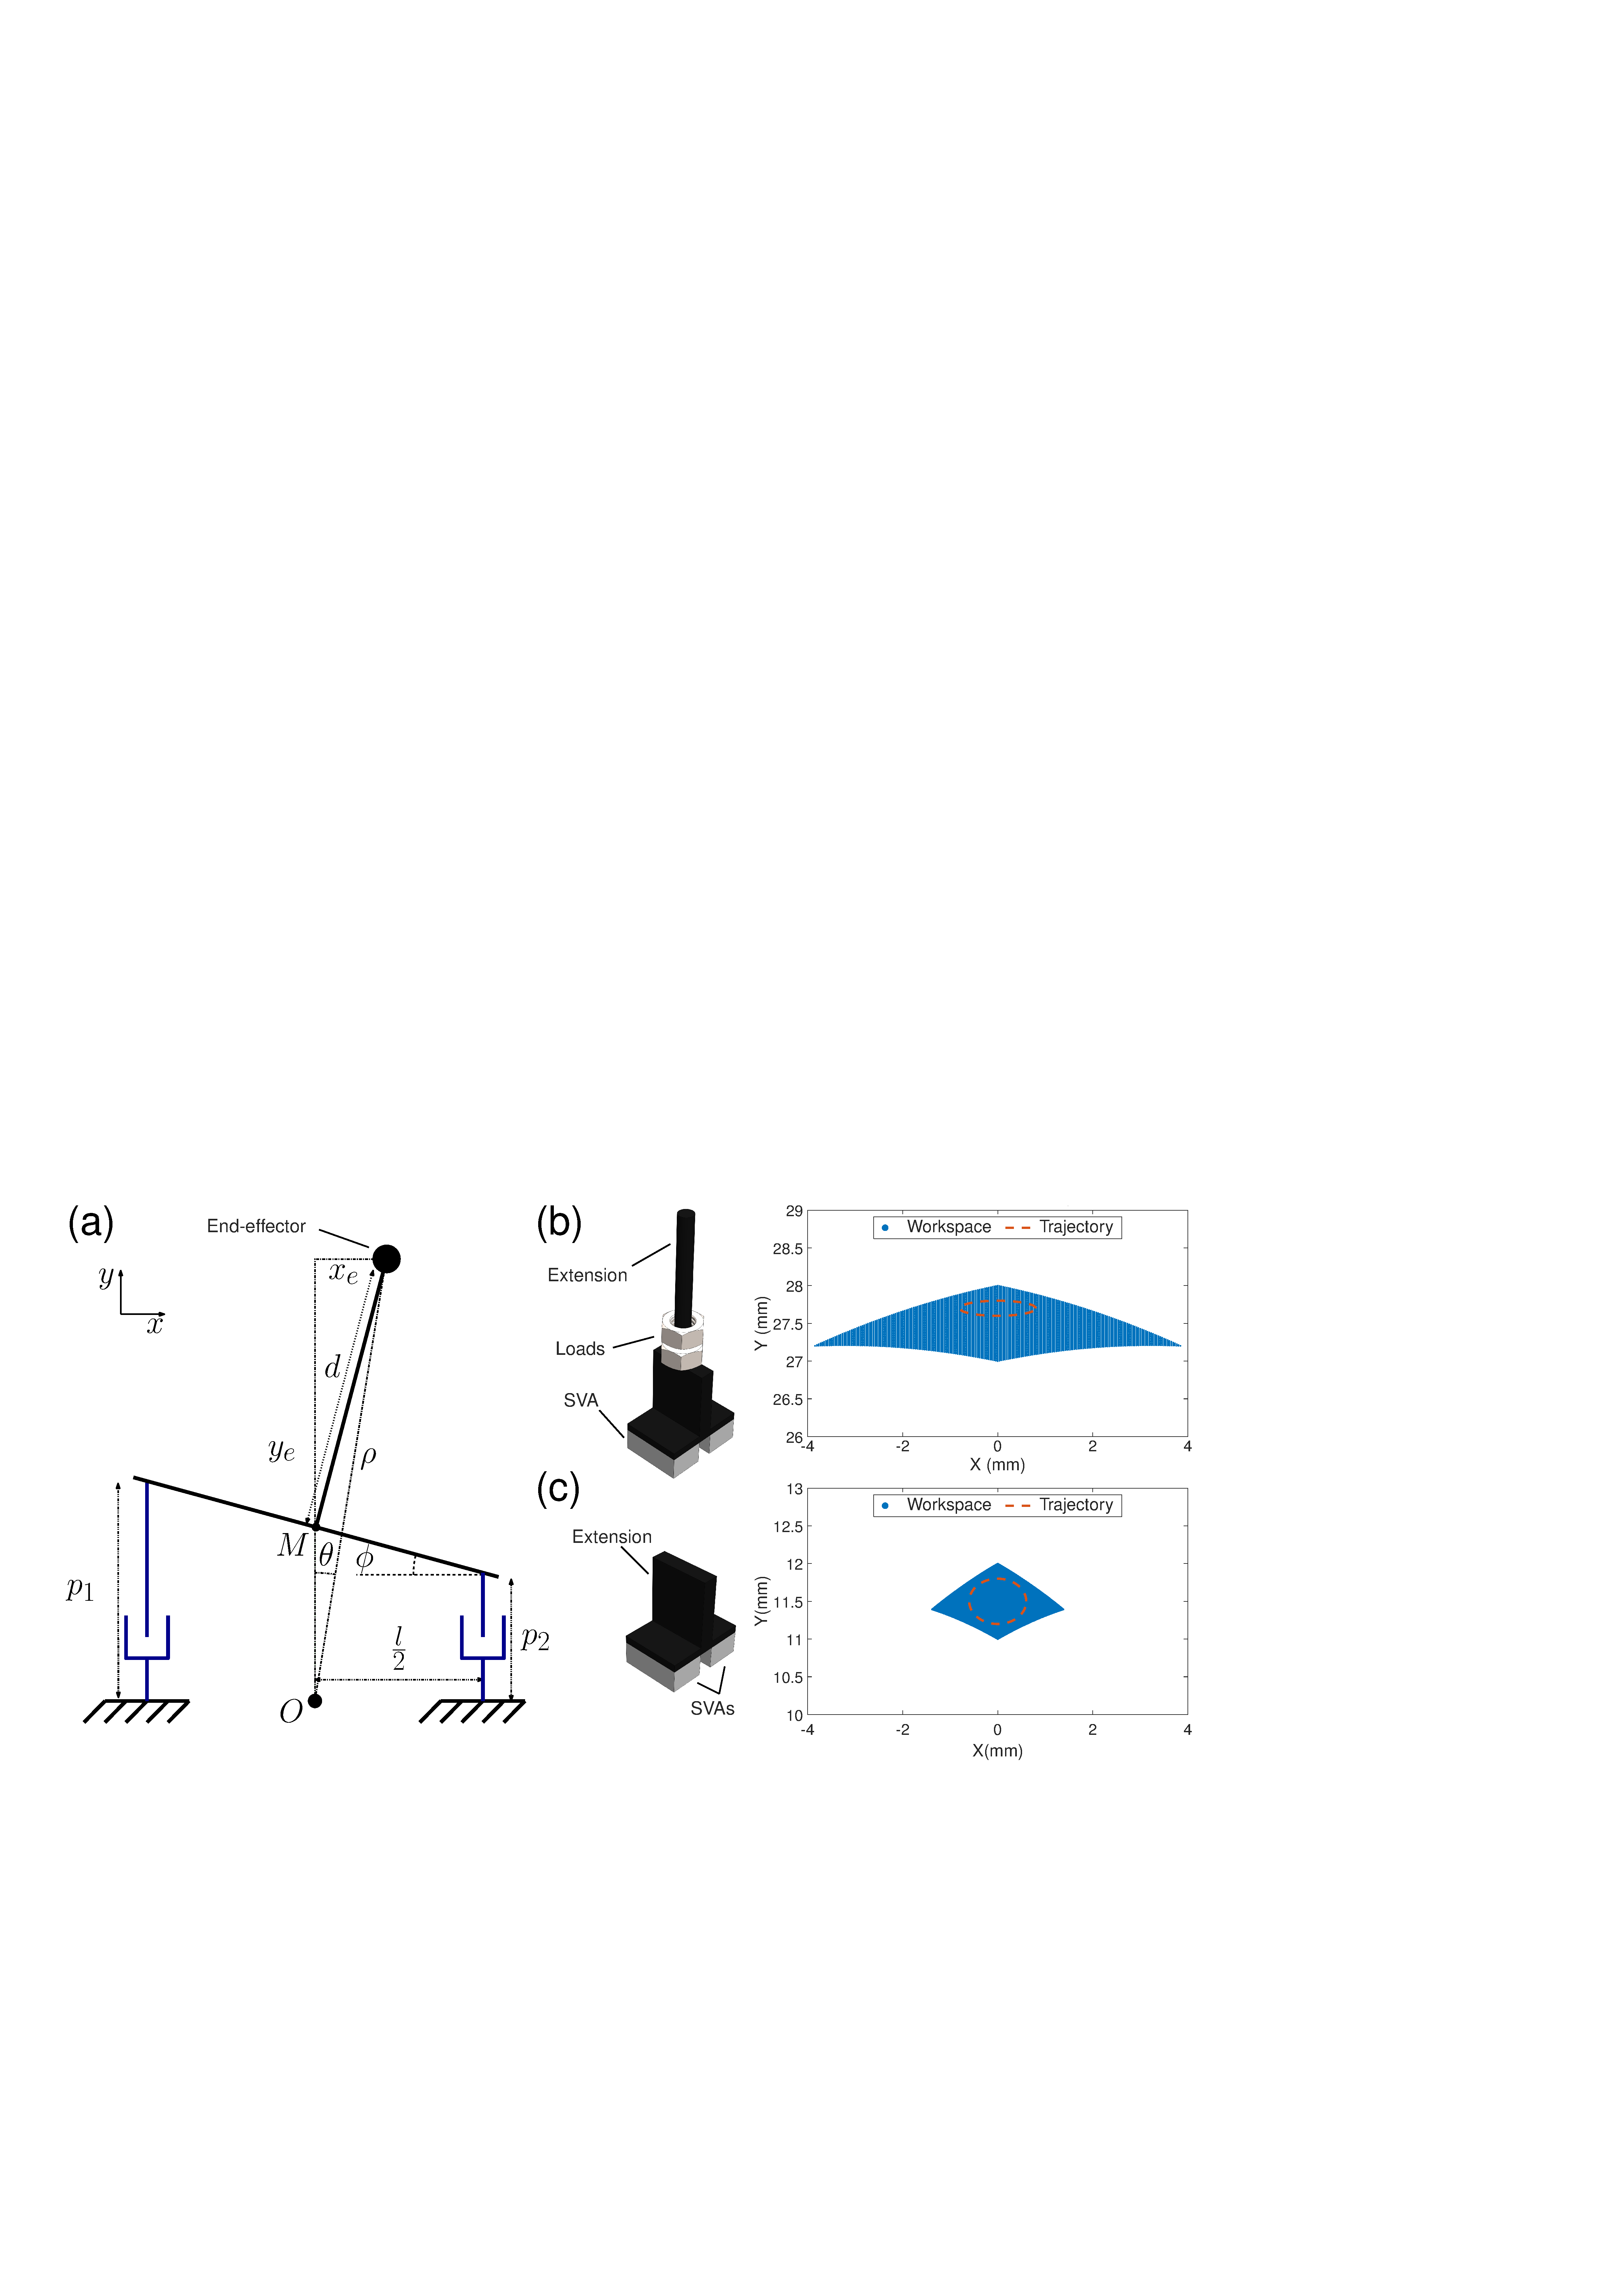
\includegraphics[width=\textwidth]{Path_Picture_New_Eleven.pdf}
    \caption[Schematic and workspace of the manipulator]{Schematic and workspace of the manipulator. (a) The 2-DOF parallel mechanism model with two prismatic joints. (b), (c) Workspaces for extensions with lengths $d=25$\,mm and $d=9$\,mm, respectively, with exemplar elliptical trajectories overlaid in red. Extra loads are added to the longer extension in (b) to test the robustness of the controller in experiment.}
    \label{fig:Path}
\end{figure}
 
To derive manipulator tip kinematics and  workspace, the SVAs are modeled as two prismatic joints, as illustrated in Fig.~\ref{fig:Path}a. The T-shaped extension is assumed to be rigid compared to the SVAs that are rigidly attached to the extension and circuit board. The SVAs are modeled as linear contractile elements since only one dimension of their volumetric shape change influences the displacement of the manipulator. Thus, with two prismatic actuators connected in parallel, the manipulator may be considered a 2-DOF mechanism. As shown in Fig.~\ref{fig:Path}a, we define $p_1$ and $p_2$ as the linear displacement of each SVA. These values vary between 3\,mm in inactivated SVA to 2\,mm when activated by the embedded Joule heaters;
$l=$6.5\,mm is the spacing between SVAs, $d$ is the length of the extension, and $\phi$ shows the extension's angle from the horizontal axis. We assume point $M$'s displacement in the $x$ direction is negligible~(Fig.~\ref{fig:Path}a).  The forward kinematics of the manipulator may be computed geometrically for the manipulator tip's, $\vect{p}_e$, in Cartesian coordinates, $x_e$ and $y_e$, in the reference frame with origin $O$, according to
%\dma{WHY ALL THE VSPACES?  THE TEMPLATE SPECIFIES THE SPACING.}]\azy{I assume they are from the shortened version-6 pages one}
\begin{align}
\vect{p_e}  &= \begin{bmatrix}x_e & y_e\end{bmatrix}^T,~~\phi = \arctan(\dfrac{p_1-p_2}{l}),\\
x_e &= d \sin(\phi),~~y_e= d \cos(\phi) + \dfrac{p_1+p_2}{2}.
\end{align}
The polar coordinates $\rho$ and $\theta$ of the manipulator's tip in this reference frame (see Fig.~\ref{fig:Path}a) are given by  

\begin{align}
\rho &=  \sqrt{x_e^2 + y_e^2},~~\theta = \arctan \left(\dfrac{x_e}{y_e}\right).
\end{align}
 
As illustrated in Fig.~\ref{fig:setup}c, if both SVAs are activated simultaneously with the same input voltage, then the manipulator's tip moves along the $\rho$-axis at a constant $\theta$; if only the left or right SVA is activated, then the tip undergoes an angular displacement at a constant $\rho$. Other SVA activation patterns produce a combination of displacements in both $\rho$ and $\theta$. 
% The SVAs used in this work have initial displacements of $p_1 = p_2 = 3$\,mm, and they have a maximum contraction of $p_1 = p_2 =$ 2\,mm when activated by the embedded Joule heaters. \dma{REVIEW TO SHORTEN}The spacing between them is $l =$ 6.5\,mm.
Two different extensions with lengths of $d = 25$\,mm and $d=9$\,mm were fabricated and tested, and their workspaces are shown in  Figs.~\ref{fig:Path}b and c, respectively. The longer extension is used to amplify the motion of each actuator, resulting in a larger workspace and making the controller performance easier to measure and evaluate. Extra loads may be added to the shaft of the longer extension, as shown in the left image in Fig.~\ref{fig:Path}b, in order to experimentally test the robustness of the controller. The shorter extension, by contrast, supports higher loads on the tip during trajectory tracking, as demonstrated in the payload transport application in Section \ref{sec:payload}.


\subsection{Linear State-Space Model}

As explained in the last section, the displacements of the SVAs and manipulator tip are not decoupled, since the T-shaped extension connecting the actuators to the tip establishes a rigid kinematic transformation from the prismatic motion of the actuators to the 2-DOF planar motion of the end-effector.
% Thus, the manipulator is similarly modeled as a multivariable control system with two inputs and two outputs, where the inputs are the voltages applied to the SVAs ($V_1$, $V_2$) and the outputs are the tip's position in polar coordinates ($\rho$, $\theta$). 
We model this control system using a two-dimensional linear state-space representation, which enables the implementation of a variety of control methods. Defining $\vect{x}(t) \in \mathbb{R}^{4\times1}$ as the vector of unknown system state variables at time $t$, $\dot{\vect{x}}(t)$ as the vector of time derivatives of the state variables, %as the derivative of the states with respect to time, 
$\vect{u}(t)=[V_1(t) \quad V_2(t)]^T$ as the vector of inputs, and $\vect{y}(t)=[\theta(t) \quad \rho(t)]^T$ as the vector of outputs, the state-space model is given by
% \dma{ISN'T THIS STANDARD?} \spr{yes, but we refer to this model later}
\begin{align}
\dot{\vect{x}}(t)&= \vect{A}\vect{x}(t)+\vect{B}\vect{u}(t), \nonumber\\
\vect{y}(t)&= \vect{C}\vect{x}(t)+\vect{D}\vect{u}(t)\label{eq:2Dmodel} 
\end{align}
where the matrices $\vect{A}$, $\vect{B}$, $\vect{C}$, and $\vect{D}$ must be determined for each extension (25\,mm and 9\,mm), separately. Since the state variables of the model are not necessarily measurable, it is crucial to understand the relationship between various input-output models and state-space models in order to accurately identify the state-space model from input-output data~\cite{Lim1998}. To find and select a model that best represents the system's behavior, a number of models were considered including state-space models of different dimensionalities.
% polynomial or nonlinear representations. However, since the state-space model 
the 2-input 2-output showed a good fit to the data and also directly provides the unknown matrices that are required for  designing the controller, we identified the system using a state-space model. $\vect{A}$, $\vect{B}$, $\vect{C}$, and $\vect{D}$ were identified by applying black-box system identification to a set of time series input-output data according to~\cite{Ljung2001}, using the MATLAB System Identification Toolbox. The identified matrices for the 25\,mm extension were found to be: 

\begin{align*}
\vect{A} &=\begin{bmatrix} 
   -0.0007 &  -0.0301  &  0.0444 &   6.0548\\
   -0.0016 &  -0.0623  &  0.0254 &  -1.4325\\
   -0.2613  &  0.6580  &  7.2633 &-374.9846\\
   -0.0243  &  0.1643  &  3.0590 & -44.3024
    \end{bmatrix},\\
\vect{B} &=\begin{bmatrix}
    0.0001 &   0.0003\\
   -0.0000 &  -0.0001\\
   -0.0051 &  -0.0232\\
   -0.0001 &  -0.0042\\
    \end{bmatrix},\\
\vect{C} &=\begin{bmatrix}  
 1.1446  & -0.0046  & -0.0020  &  0.0034\\
-1.1431  & -3.5368  &  0.0020 &  -0.0534
    \end{bmatrix},\\
\vect{D} &=\begin{bmatrix}
     0  &   0\\
     0  &   0
    \end{bmatrix}.
\end{align*}
 
Multiple input-output datasets were gathered across various ranges of amplitudes and frequencies to find a state-space model. Among all the input signals, the fastest signal that permitted the hydrogel actuators to respond across their full temperature range was selected as the primary modeling input. Figure~\ref{fig:sim}a plots two selected input voltages among the data set that were experimentally applied to the SVAs which covers the tip workspace and depicts a 50\%  shift in the SVAs' input signal. Since the hydrogel-based SVAs have a relatively slow response, especially during their cooling phase, they were actuated from a starting point of half-actuation (50\%) in order to improve both the speed and tracking performance of the manipulator and the signal reaches the minimum and maximum values during the cycle. Fig.~\ref{fig:sim}b displays the resulting displacement of the manipulator tip and the outputs of the identified model \eqref{eq:2Dmodel} for the same inputs. These figures, which are a comprehensive example of comparison between the actual data and the identified model output, show that the model outputs $\rho$ and $\theta$ follow the corresponding measured output values throughout the duration of the experiment, with the NMAE for $\rho$ and $\theta$ given by 0.026\,mm (5.7\%) and 0.008\,rad (6.6\%), respectively. The NMAE value remains below 10\% for other tested data sets. Thus, our linear state-space model of the entire mechanism is sufficiently accurate to use in the design of controllers for the manipulator, despite the difficult-to-characterize nonlinear dynamics of the hydrogel actuators themselves.

\begin{figure}[h]
\centering
{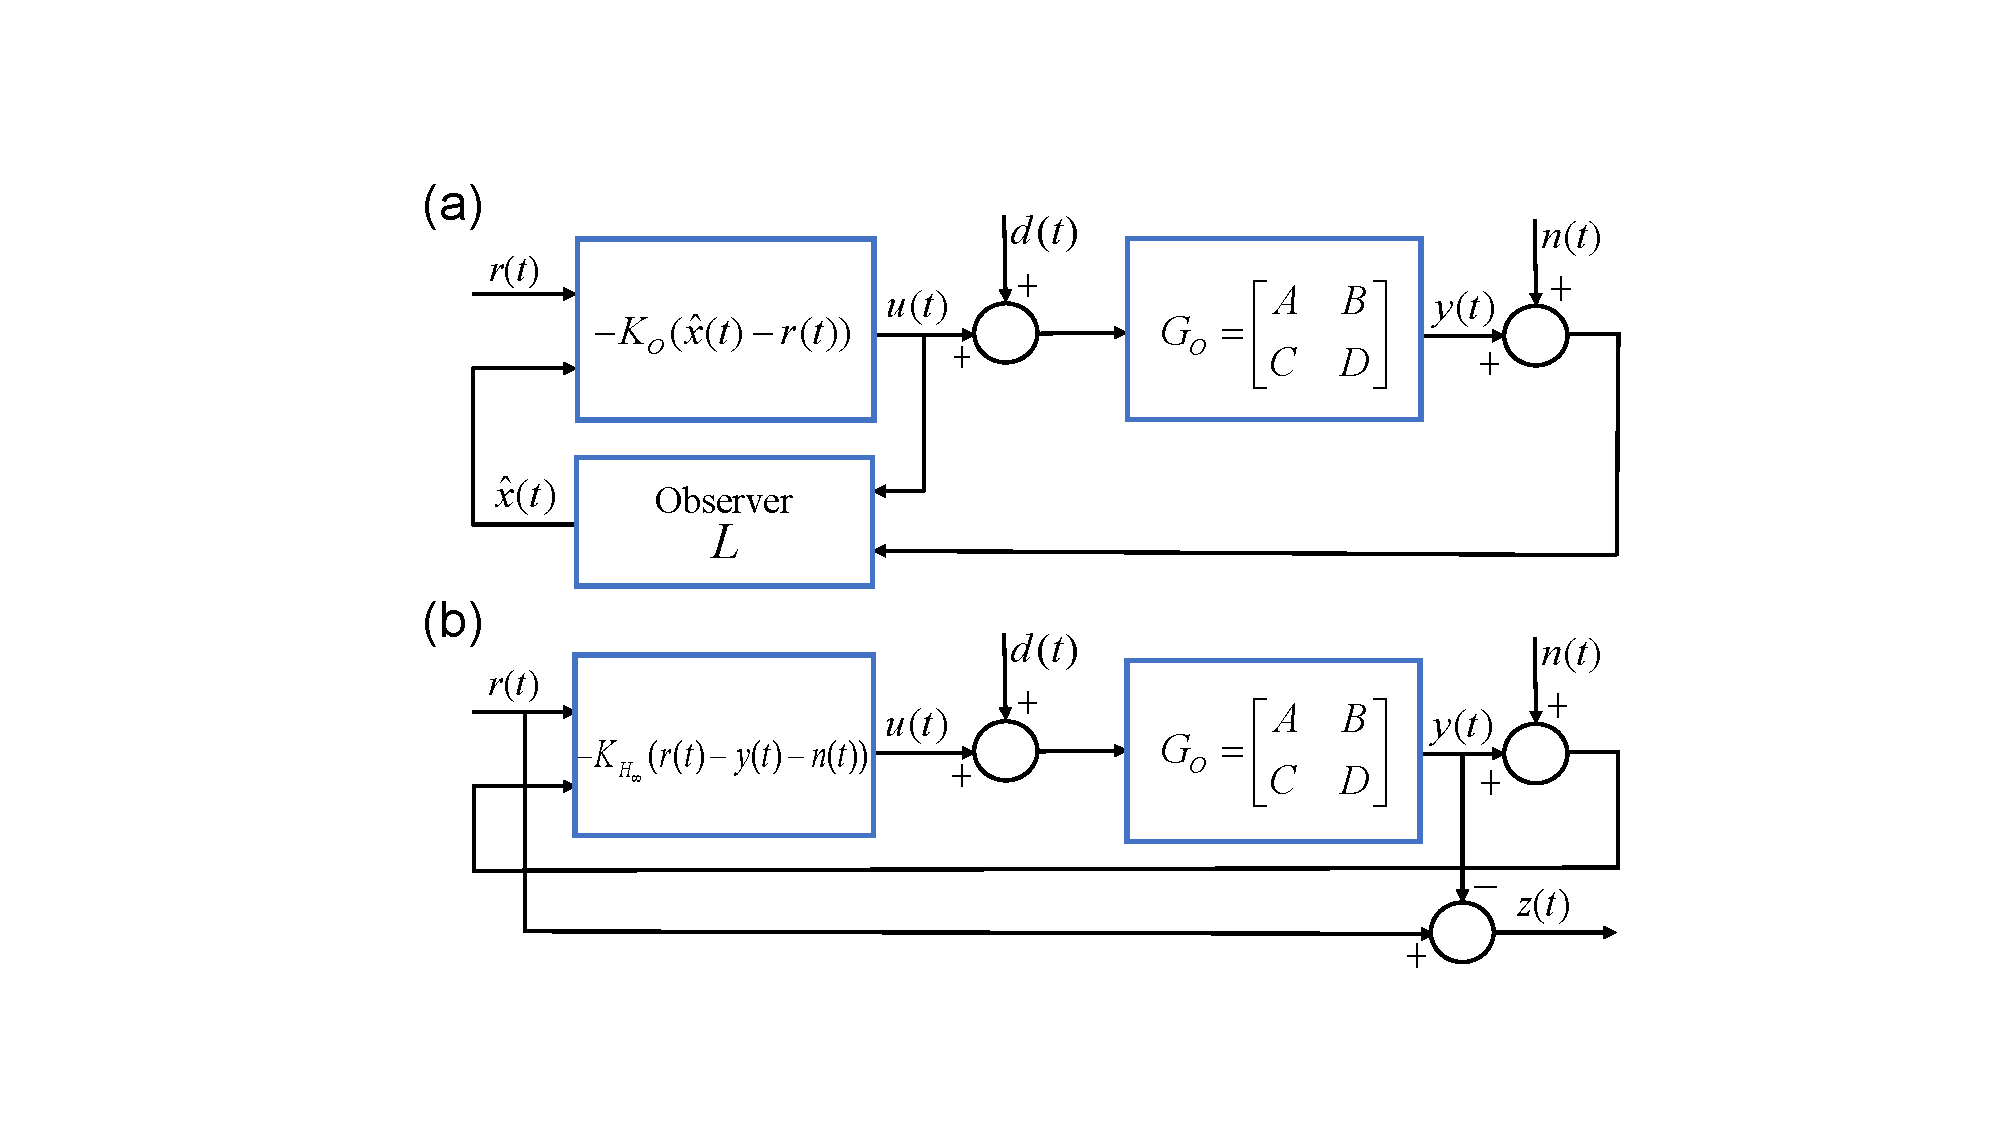
\includegraphics[width=\textwidth]{output-feedback-control_block_final.pdf}}
\caption[Block diagrams of the proposed output-feedback controllers]{Block diagrams of the proposed output-feedback controllers with state-space representation in the tracking framework~\cite{Skogestad2007}. (a) Observer-based controller. (b) $H_\infty$-optimal controller.} \vspace{-0.5cm}
\label{fig:control_block}
\end{figure}

\section{Controller Design} 

It can be shown that the open-loop state-space model~\eqref{eq:2Dmodel}, which has the corresponding transfer function $\vect{G}_o(s)$, is stable, controllable, and observable. In this section, we design two trajectory tracking controllers based on this state-space model, an observer-based output-feedback controller and an $H_{\infty}$-optimal output-feedback controller. Block diagrams of the controllers are illustrated in Fig.~\ref{fig:control_block}. Both controllers are designed to track a reference trajectory $\vect{r}(t) \in \mathbb{R}^{2\times1}$ while attenuating the effects of noise, denoted by $\vect{n}(t)\in \mathbb{R}^{2\times1}$, and external disturbances, denoted by $\vect{d}(t)\in \mathbb{R}^{2\times1}$.

\subsection{Observer-based output-feedback controller}

In this type of controller, an observer is designed to compute an estimate  $\hat{\vect{x}}(t)$ of the unknown system state vector $\vect{x}(t)$ from the control input $\vect{u}(t)$ and the output $\vect{y}(t)$. The control input is defined as 
\begin{align}
&\vect{u}(t)=-\vect{K}_O\left(\hat{\vect{x}}(t)-\vect{r}(t)\right), \label{eq:obs-ctl-law}
\end{align}
where $\vect{K}_O \in \mathbb{R}^{2\times4}$ is the feedback gain matrix, which can be computed as though all state variables are measurable, depending only on the $\vect{A}$ and $\vect{B}$ matrices. With this control input, the observer is given by 

\begin{align}
&\hat{\dot{\vect{x}}}(t)=(\vect{A}-\vect{B}\vect{K}_O-\vect{LC})\hat{\vect{x}}(t)+\vect{L}\vect{y}(t), \label{eq:obs-estimate}
\end{align}
where $\vect{L}\in \mathbb{R}^{4\times2}$, the observer gain matrix, must be defined such that $\vect{A-LC}$ is a Hurwitz matrix~\cite{Aastrom2010}.
The following $\vect{K}_O$ and $\vect{L}$ matrices were computed for the 25\,mm extension: 

% \spr{(should we explain how?)} \azy{I think as it is the typical observer calculations we don't need to}
\begin{align*}
\vect{K}_O &=\begin{bmatrix}  
            -3.8929  & 2.3760   &  -0.1061  &  0.2888\\
             3.6672  & -0.9670  &   0.0949  & -0.2706
    \end{bmatrix},\\
\vect{L} &=\begin{bmatrix}
           18.5160 &  -21.9676\\   
            0.1852 &  -7.7968\\
           -0.0051 &   0.0232\\
           -0.0649 &   0.0042\\
    \end{bmatrix}.
\end{align*}

\subsection{$H_\infty$-optimal output-feedback controller}

The $H_\infty$-optimal controller is designed using Linear Matrix Inequality (LMI) methods~\cite{Duan2013a,Boyd1994}; MATLAB's YALMIP toolbox~\cite{Lofberg2004} is then used to solve the optimization problem numerically. rev{The interconnected system $S(\vect{K}_{H_{\infty}},\vect{G}_o)$ of the optimal gain matrix $\vect{K}_{H_{\infty}}\in \mathbb{R}^{2\times2}$ and the open-loop system $\vect{G}_o(s)$, with external input defined as $\vect{w}=~[\vect{r}^T~\vect{d}^T~\vect{n}^T]^T \in \mathbb{R}^{6\times1}$ and external output $\vect{z}=\vect{r}-\vect{y}$, represents the closed-loop system with the ${H_{\infty}}$ gain:} \vspace{2mm}
\begin{align}
\norm{\vect{z}}_{L_2} ~\leq~ \norm{S(\vect{K}_{H_{\infty}},\vect{G}_o)}_{H_{\infty}} \norm{\vect{w}}_{L_2}.
\end{align}

The optimal gain matrix $\vect{K}_{H_{\infty}}$ is obtained as the solution to an optimization problem that minimizes the effect of the external input ($\vect{w}$) on the external output ($\vect{z}$). We can prove that the ${H_{\infty}}$ gain is bounded using the bounded-real lemma~\cite{Boyd1994}~(see Appendix). The control law is designed in the the output-feedback tracking structure: \vspace{2mm}
\begin{align}
\vect{u}(t)=-\vect{K}_{H_\infty}(\vect{r}(t)-\vect{y}(t)-\vect{n}(t)). \label{eq:Hinf-ctl}
\end{align}

The gain matrix for the 25\,mm extension %manipulator 
was computed as \vspace{2mm}
\begin{align*}
\vect{K}_{H_{\infty}} &=\begin{bmatrix}  
           -1.7371  &  2.9015 \\
           -0.3775  & -2.4158  
    \end{bmatrix}.
\end{align*}


\begin{figure*}[t]
\centering
    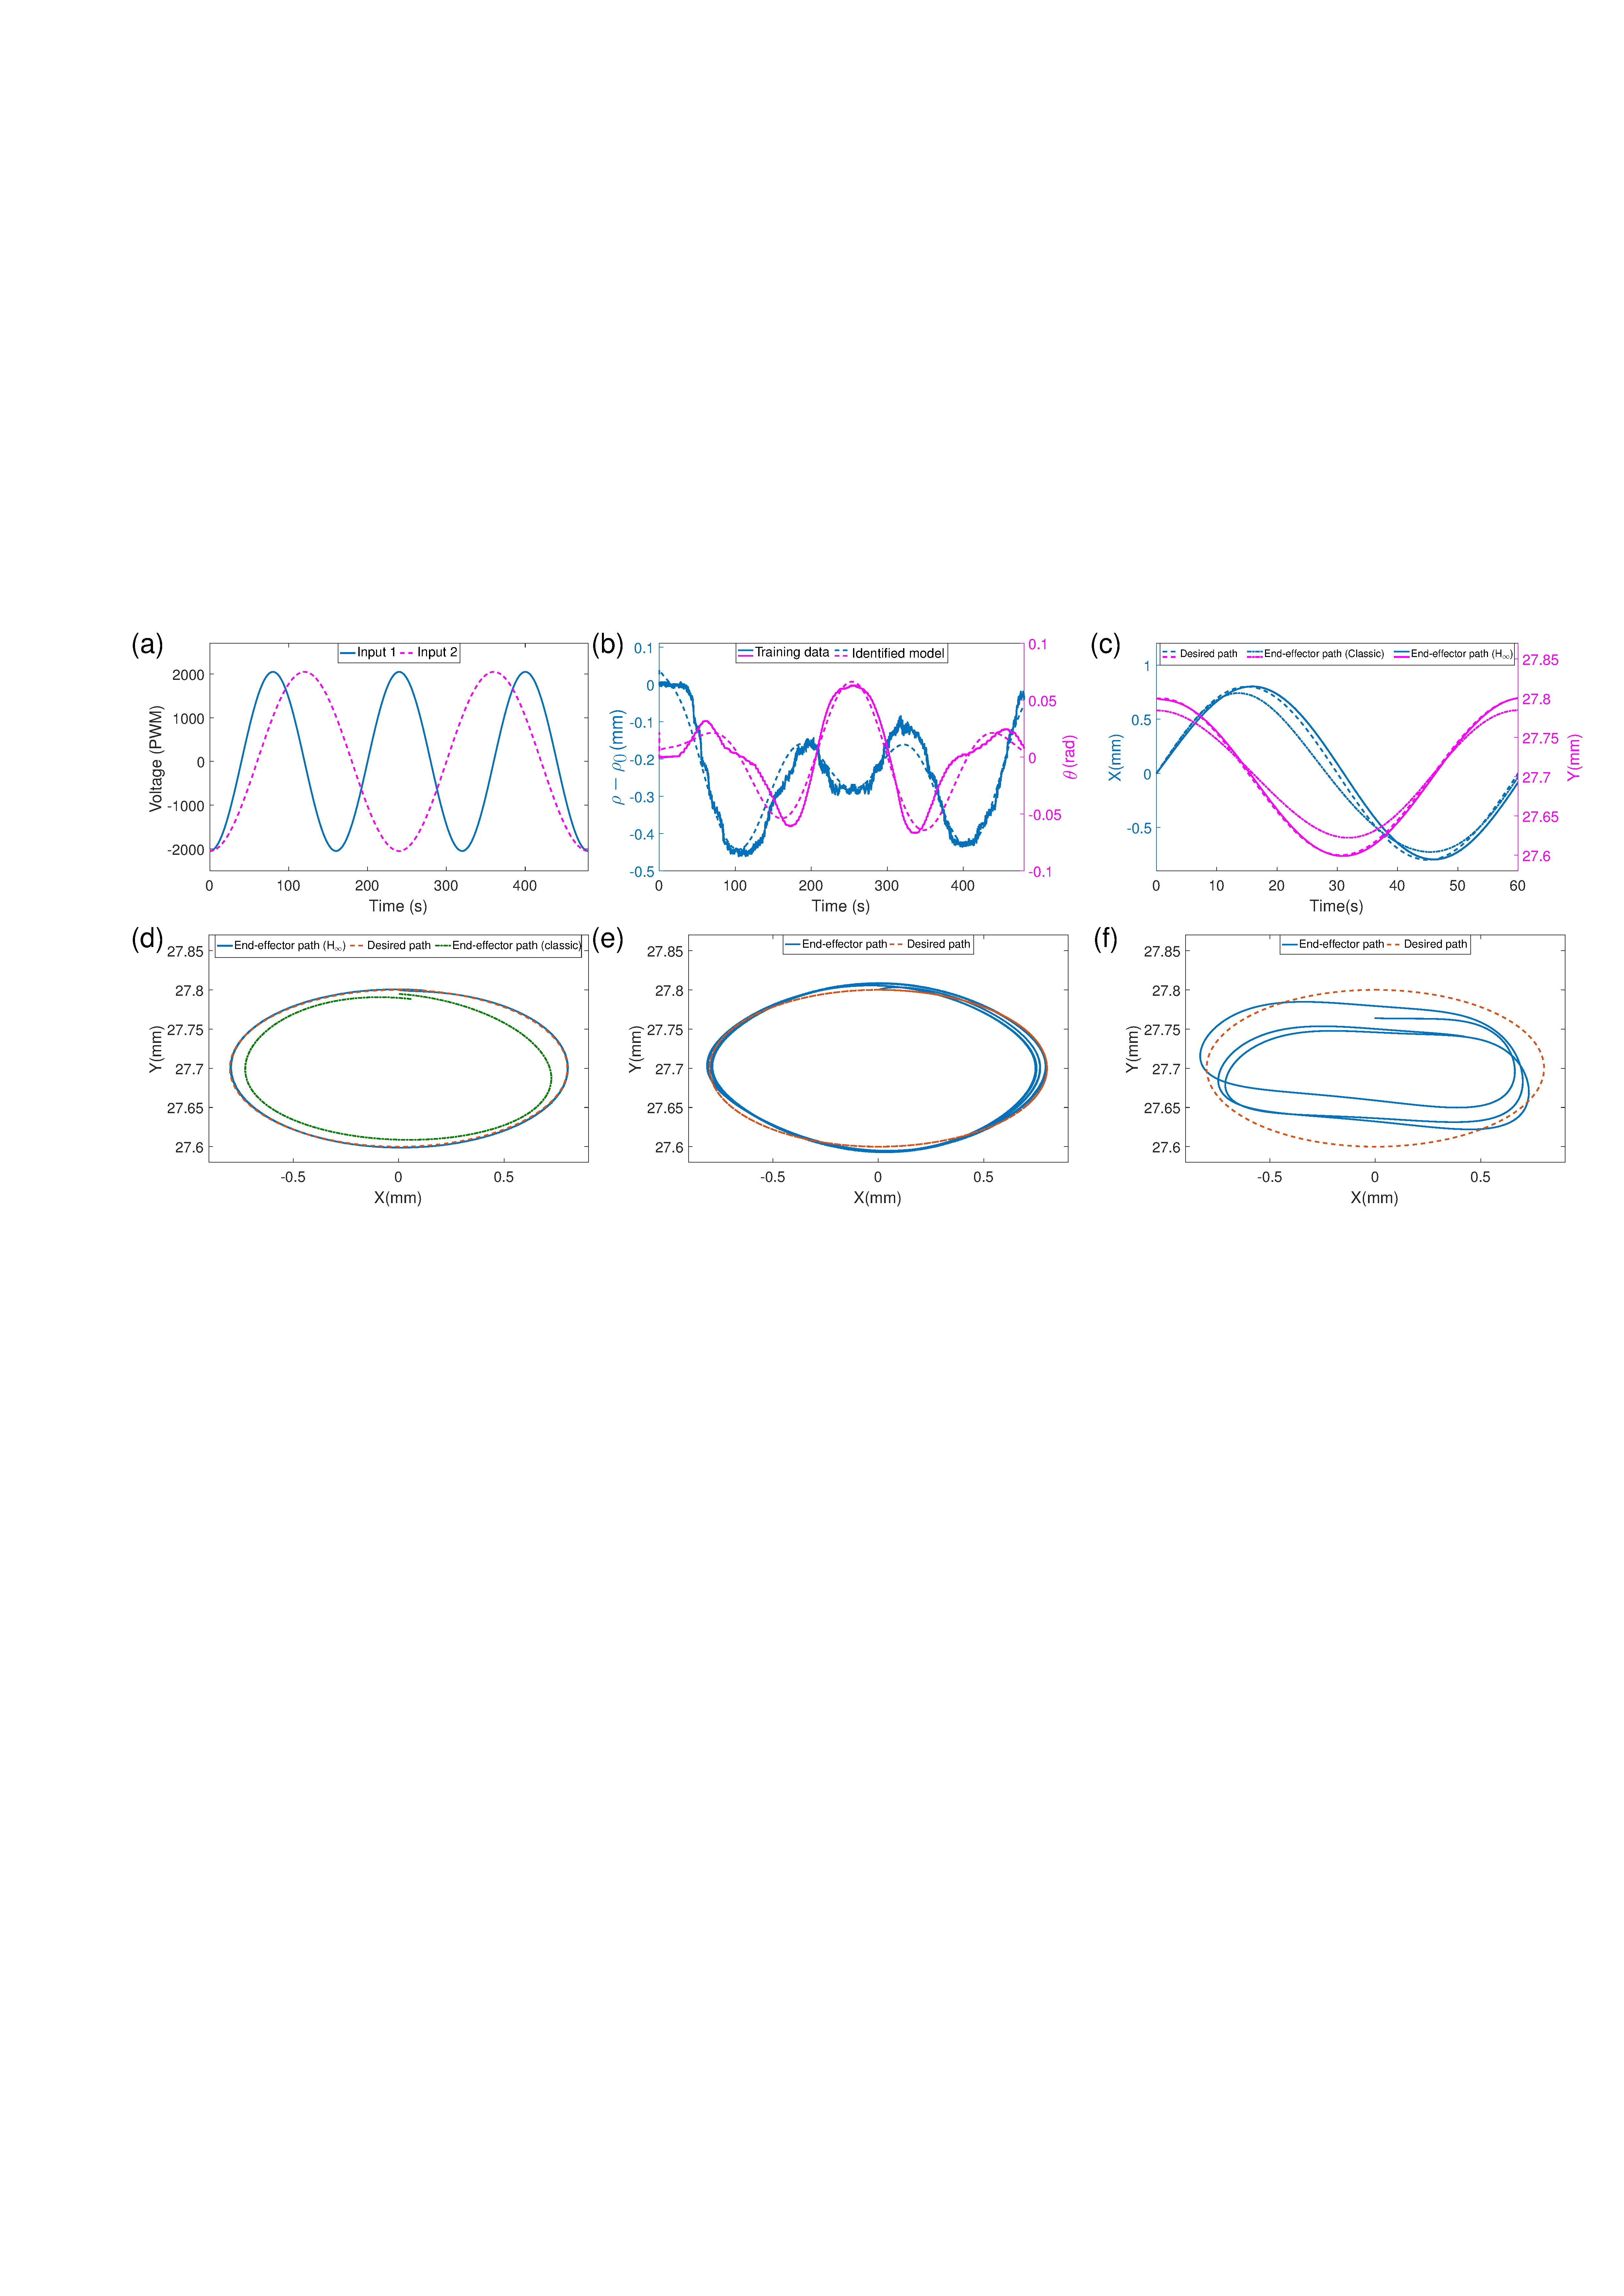
\includegraphics[width=\textwidth]{Figure_Sim_6.pdf}
    \caption[Simulation results of the controller]{Simulation results. (a) 12-bit PWM waveform applied to the SVAs during training. (b) System output and model fitted from training. (c) The $x$ and $y$ coordinates of the manipulator tip over time for the $H_\infty$-optimal and Observer-based controllers, tracking an ellipse. (d) The $x$-$y$ trajectory of the tip during the simulation in (c).
    (e) $H_\infty$-optimal controller with noise and disturbance. (f) Observer-based controller with noise and disturbance.} \vspace{-0.5cm}
\label{fig:sim}
\end{figure*}

%--------------------------------------------------------
\section{Results and Discussion}
% \dma{REVIEW WITH DMAs}

In this section, we study the performance of $H_\infty$ and observer controllers for trajectory tracking. An elliptical reference trajectory is used, defined by

\begin{align}
\vect{r}(t)= \begin{bmatrix} \alpha\sin\left(\frac{2\pi}{60}t\right) & \beta+\gamma\cos\left(\frac{2\pi}{60} t\right)
\end{bmatrix}^T. 
\end{align}
where $\alpha=0.8$, $\beta=27.7$, and $\gamma=0.1$ for the 25\,mm extension, and $\alpha=0.6$, $\beta=11.5$, and $\gamma=0.3$ for the 9\,mm extension, to ensure that each path lies in the workspace of its corresponding manipulator (see Fig.~\ref{fig:Path}). The manipulator's tracking performance degraded at frequencies of higher than one cycle per minute.% (Figs.~\ref{fig:Control_outputs}g and~\ref{fig:Control_outputs}h).

%\dma{REMOVE THIS:}
%The $H_\infty$-optimal controller is then implemented experimentally on the manipulator and evaluated for different reference trajectories and loads. Finally, we present an application of the $H_\infty$-optimal controller to payload transport by an array of four manipulators with 9\,mm extensions.

%--------------------------

\begin{table}[t]
\centering
\caption{N(MAE) of controller performance in simulation (in mm).}
\begin{tabular}{c c c c c c}
\hline
Controller&Noise $\&$& $x$ & $y$& $x-y$& $x-y$\\
           &disturbance& MAE & MAE & MAE & NMAE ($\%$)\\
\hline
% $H_{\infty}$       & 9\,mm & 0.044 & 0.017 & 0.055 & 4.1\\
% \rev{Observer}            & 9\,mm & 0.074 & 0.027 & 0.100 & 7.4\\
$H_{\infty}$       & No & 0.045 & 0.006 & 0.052 & 3.2\\
Observer            & No & 0.065 & 0.008 & 0.079 & 4.9\\
$H_{\infty}$ & Yes & 0.047 & 0.005 & 0.055 & 3.4\\
Observer & Yes & 0.078 & 0.009 & 0.096 & 5.9\\
\hline
\end{tabular}
\label{table:sim}
\vspace{-4mm}
\end{table}

\subsection{Comparison of controllers in simulation}
The performance of the two controllers is first compared in simulation in the presence of the following disturbance and noise signals:
\begin{align}
\vect{d}(t)&= \begin{bmatrix} 0.00015\sin\left(\frac{3\pi}{60}t\right) & 0.00045\sin\left(\frac{2\pi}{60} t\right)
\end{bmatrix}^T,\\
\vect{n}(t)&= \begin{bmatrix} 0.3\sin\left(\frac{\pi}{60}t\right) & 0.3\sin\left(\frac{0.5\pi}{60} t\right)
\end{bmatrix}^T. 
\end{align}
%To compare the performance of the observer-based and $H_{\infty}$-optimal controllers, 
The manipulator with the 25\,mm extension was simulated in MATLAB Simulink, using the output-feedback tracking framework depicted in Fig.~\ref{fig:control_block} and the identified model and controller values designed in the previous section.
Figures~\ref{fig:sim}c and~\ref{fig:sim}d plot the $x$ and $y$ coordinates and the trajectory of the manipulator tip over time for one cycle (60\,s), given an elliptical reference trajectory, from each controller. 
% A similar comparison was performed for a simulated manipulator with a 9\,mm extension,~(reported in Table~\ref{table:sim}). 
To observe the effect of adding noise and disturbance in simulation, the sinusoidal functions of $\vect{n}$ and $\vect{d}$ were input to the 25\,mm manipulator. The tracking trajectories of the manipulator tip produced by each controller are compared in Figs.~\ref{fig:sim}e and~\ref{fig:sim}f, separately. Although the simulations are performed across three cycles, only one cycle is shown in the figures and used in the error comparison for clarity. The tracking error for each case is reported in Table~\ref{table:sim}.The NMAE values were computed by dividing the mean absolute error (MAE) over their corresponding range. All the values are relatively low, under 10\%, indicating accurate tracking. 

%-------------------------------------------------------

%\begin{figure*}[t]
%\centering
    %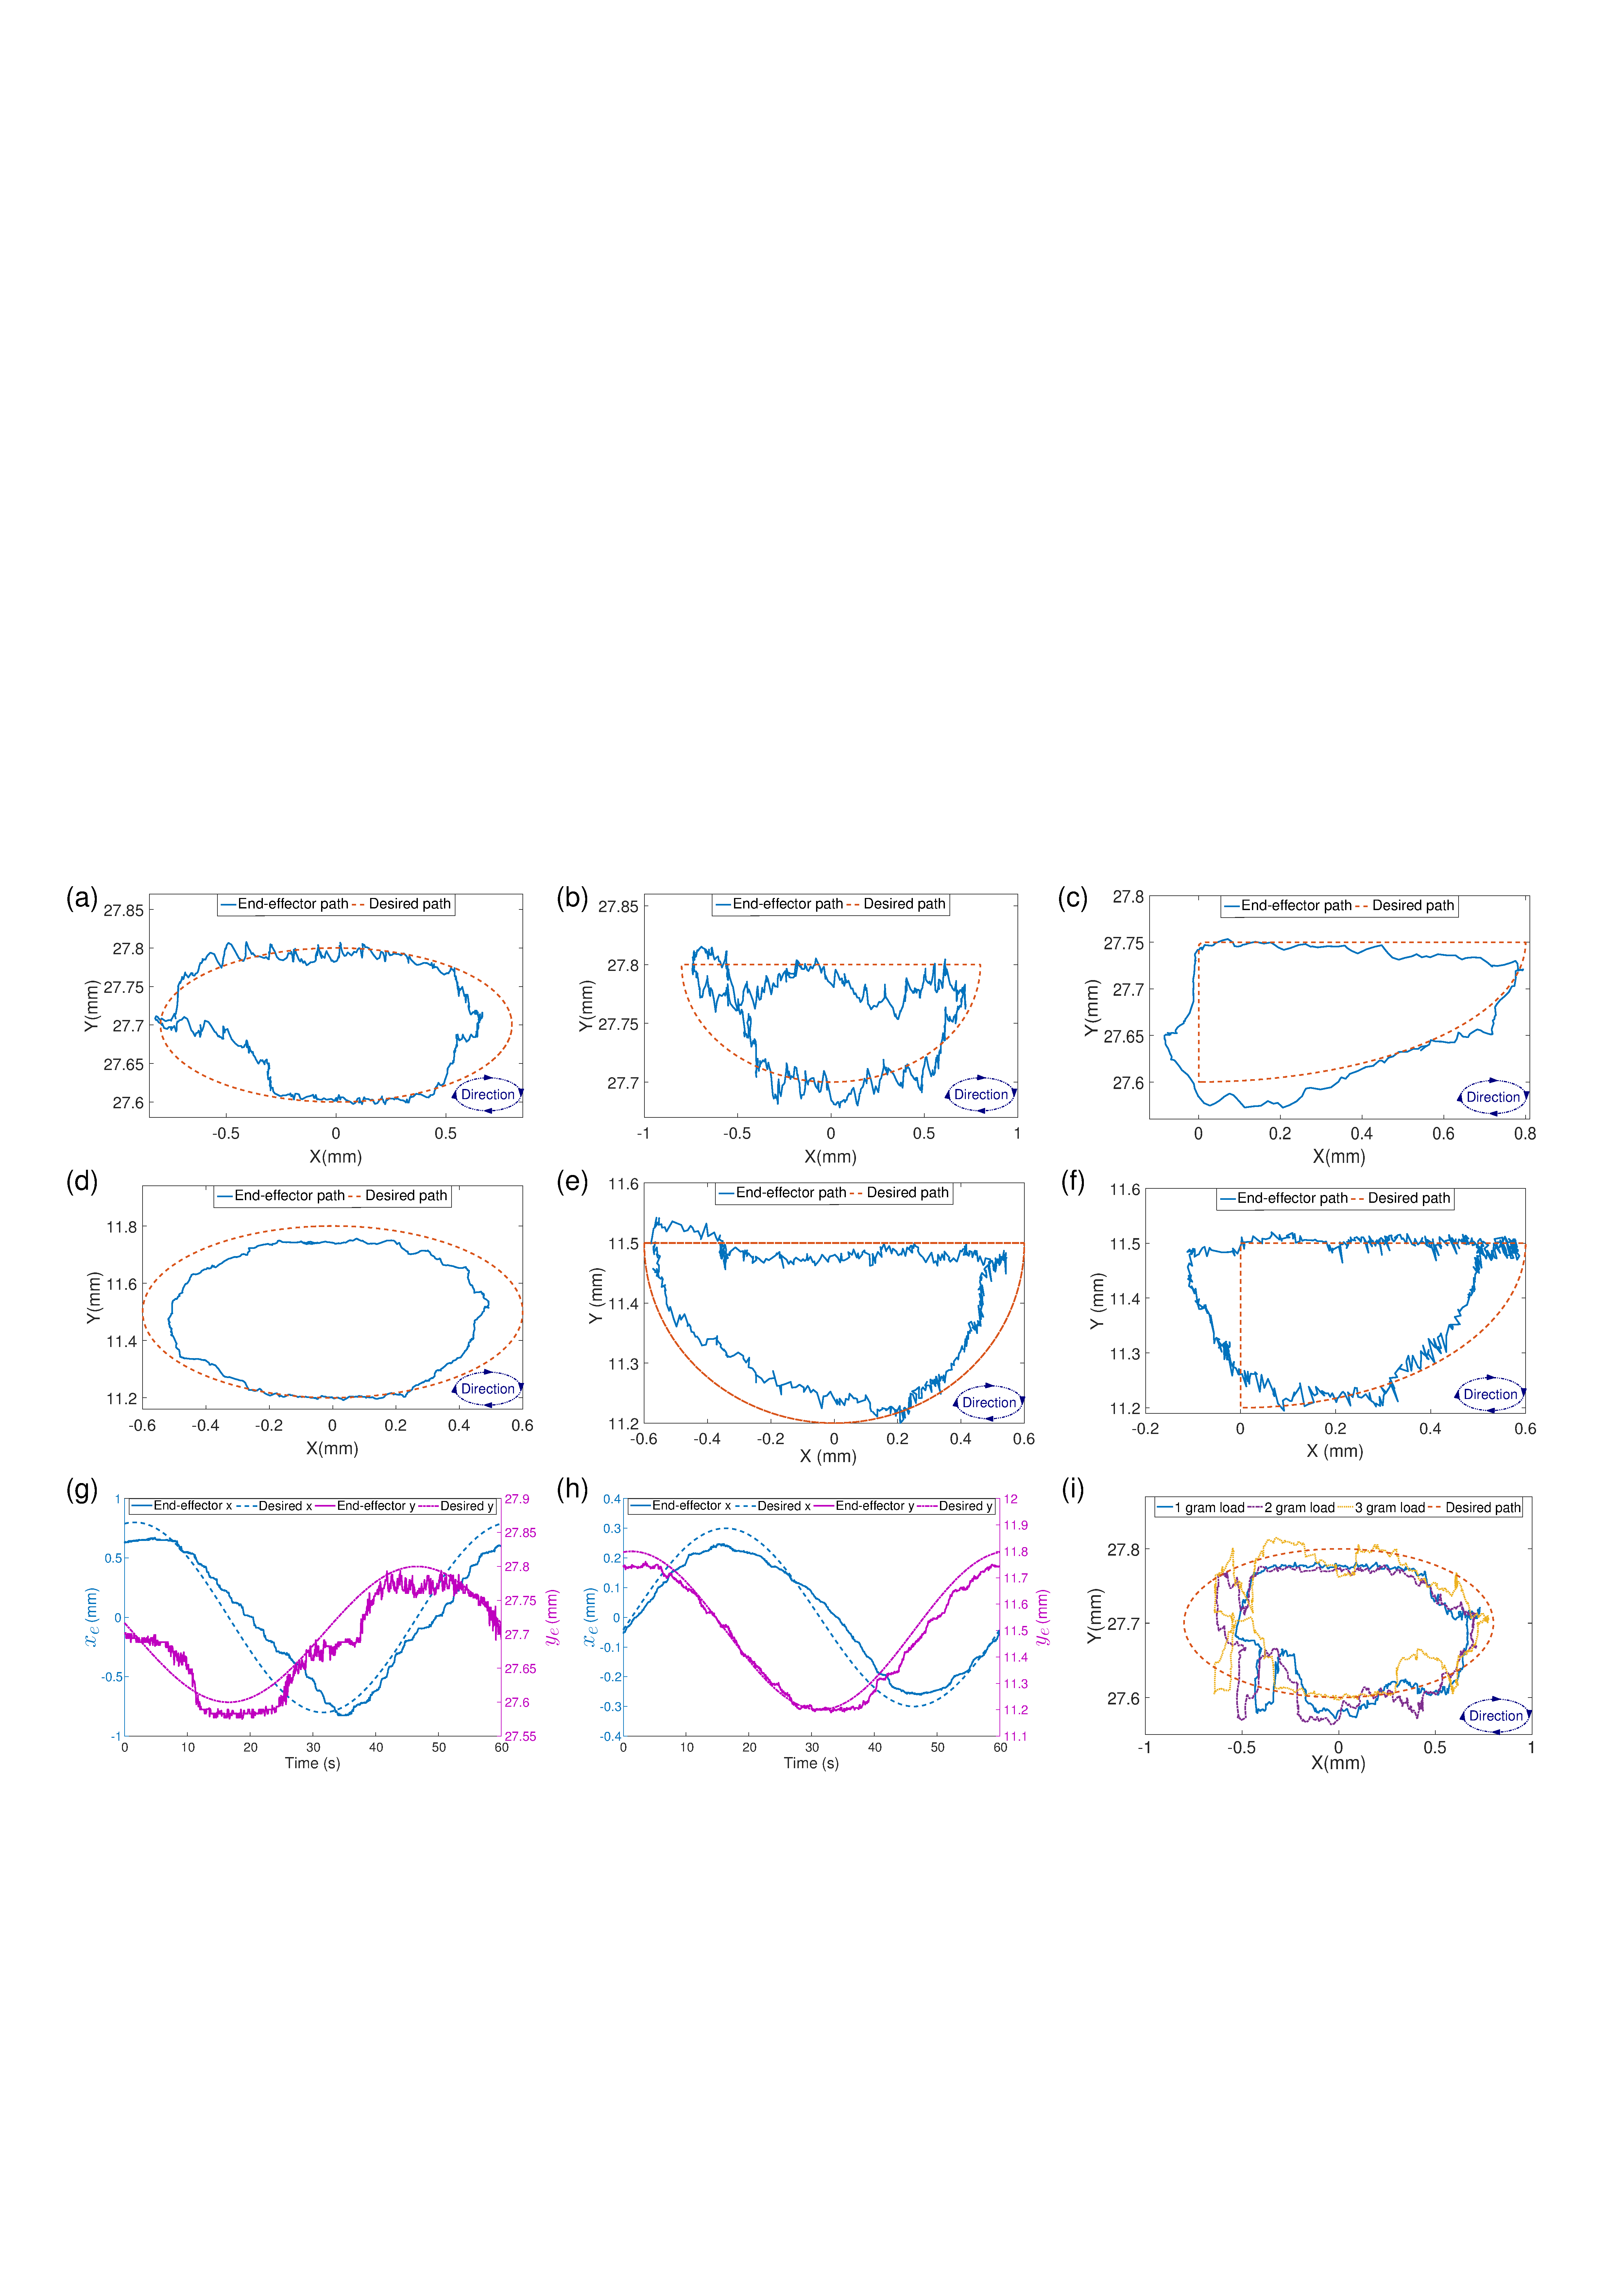
\includegraphics[width=\textwidth]{Control_Picture_New_Ten.pdf}
    %\caption[Tracking reference and experimental trajectories of  manipulator tip]{Tracking reference and experimental trajectories of  manipulator tip in Cartesian coordinates. 25\,mm manipulator tracking: (a) an elliptical trajectory; (b) a half-ellipse; (c) a quarter-ellipse. 9\,mm manipulator tracking: (d) an elliptical trajectory; (e) a half-ellipse; (f) a quarter-ellipse. (g) 25\,mm manipulator tracking an elliptical trajectory: $x,y$ coordinates over time separately. (h) 9\,mm manipulator tracking an elliptical trajectory: $x,y$ coordinates over time separately. (i) 25\,mm manipulator tracking an elliptical trajectory under 1\,g, 2\,g, and 3\,g.}
    %\label{fig:Control_outputs}
%\end{figure*}
%%--------------------------------------------------------------------
%\subsection{Experimental validation of $H_\infty$-optimal controller}
%
%Since the $H_\infty$-optimal controller exhibited higher tracking accuracy in simulation both with and without disturbance and noise, it was selected for experimental implementation. Using the designed control gain for $H_\infty$, we have implemented the output-feedback tracking framework depicted in Fig.~\ref{fig:control_block}b on the hydrogel-based manipulator (Fig.~\ref{fig:setup}). Half-ellipse and quarter-ellipse paths were also used as reference trajectories. Sources of noise in the experiment arise in the testing environment and vision-based feedback. Disturbances include modeling and manufacturing errors.  The MAE and NMAE values are reported for one cycle per trajectory in Table~\ref{table:control}, though three repeating cycles per trajectory were collected.
%
%Figure~\ref{fig:Control_outputs}a compares the trajectory of a manipulator with the 25\,mm extension driven by the controller Equation~\eqref{eq:Hinf-ctl} along an elliptical reference trajectory. Controller performance was evaluated using a half-ellipse and quarter-ellipse reference trajectory as well, to verify the ability of the controlled system to track straight lines and sharp turns (Figs.~\ref{fig:Control_outputs}b and~\ref{fig:Control_outputs}c). Figures~\ref{fig:Control_outputs}d, ~\ref{fig:Control_outputs}e ,and~\ref{fig:Control_outputs}f show the controlled position of the 9\,mm extension's tip using the same reference trajectories. Figures~\ref{fig:Control_outputs}g and~\ref{fig:Control_outputs}h illustrate the time evolution of the $x$ and $y$ coordinates separately for the two extensions.
%
%\begin{table}[t]
%\centering
%\caption{(N)MAE of $H_{\infty}$ controller performance in experiment.}\vspace{-0.25cm}
%\begin{tabular}{c c c c c c c}
%\hline
%\hspace{-2mm} $d$ & Reference & Load & $x$ & $y$ & $x-y$ & \hspace{-2mm} NMAE\\
%\hspace{-2mm} (mm) &  trajectory   & (g)  & (mm)& (mm)& (mm) & \hspace{-2mm}$\%$\\
%\hline
%\hspace{-2mm}25 & Ellipse          & - & 0.123 & 0.042 & 0.131 & \hspace{-2mm}8.1\\
%\hspace{-2mm}25 & Half Ellipse     & - & 0.119 & 0.023 & 0.123 & \hspace{-2mm}7.6\\
%\hspace{-2mm}25 & Quarter Ellipse  & - & 0.112 & 0.026 & 0.119 & \hspace{-2mm}7.4\\
%\hspace{-2mm}9 & Ellipse           & - & 0.088 & 0.033 & 0.099 & \hspace{-2mm}7.4\\
%\hspace{-2mm}9 & Half Ellipse      & - & 0.129 & 0.058 & 0.132 & \hspace{-2mm}9.8\\
%\hspace{-2mm}9 & Quarter Ellipse   & - & 0.161 & 0.061 & 0.171 & \hspace{-2mm}12.8\\
%\hspace{-2mm}25 & Ellipse          & 1 & 0.140 & 0.022 & 0.144 & \hspace{-2mm}8.9\\
%\hspace{-2mm}25 & Ellipse          & 2 & 0.162 & 0.021 & 0.162 & \hspace{-2mm}10.1\\
%\hspace{-2mm}25 & Ellipse          & 3 & 0.164 & 0.022 & 0.164 & \hspace{-2mm}10.2\\ 
%\hline
%\end{tabular}
%\label{table:control}
%\vspace{-4mm}
%\end{table}
%
%%-----------------------------------
%\begin{figure*}[t]
%\centering
%{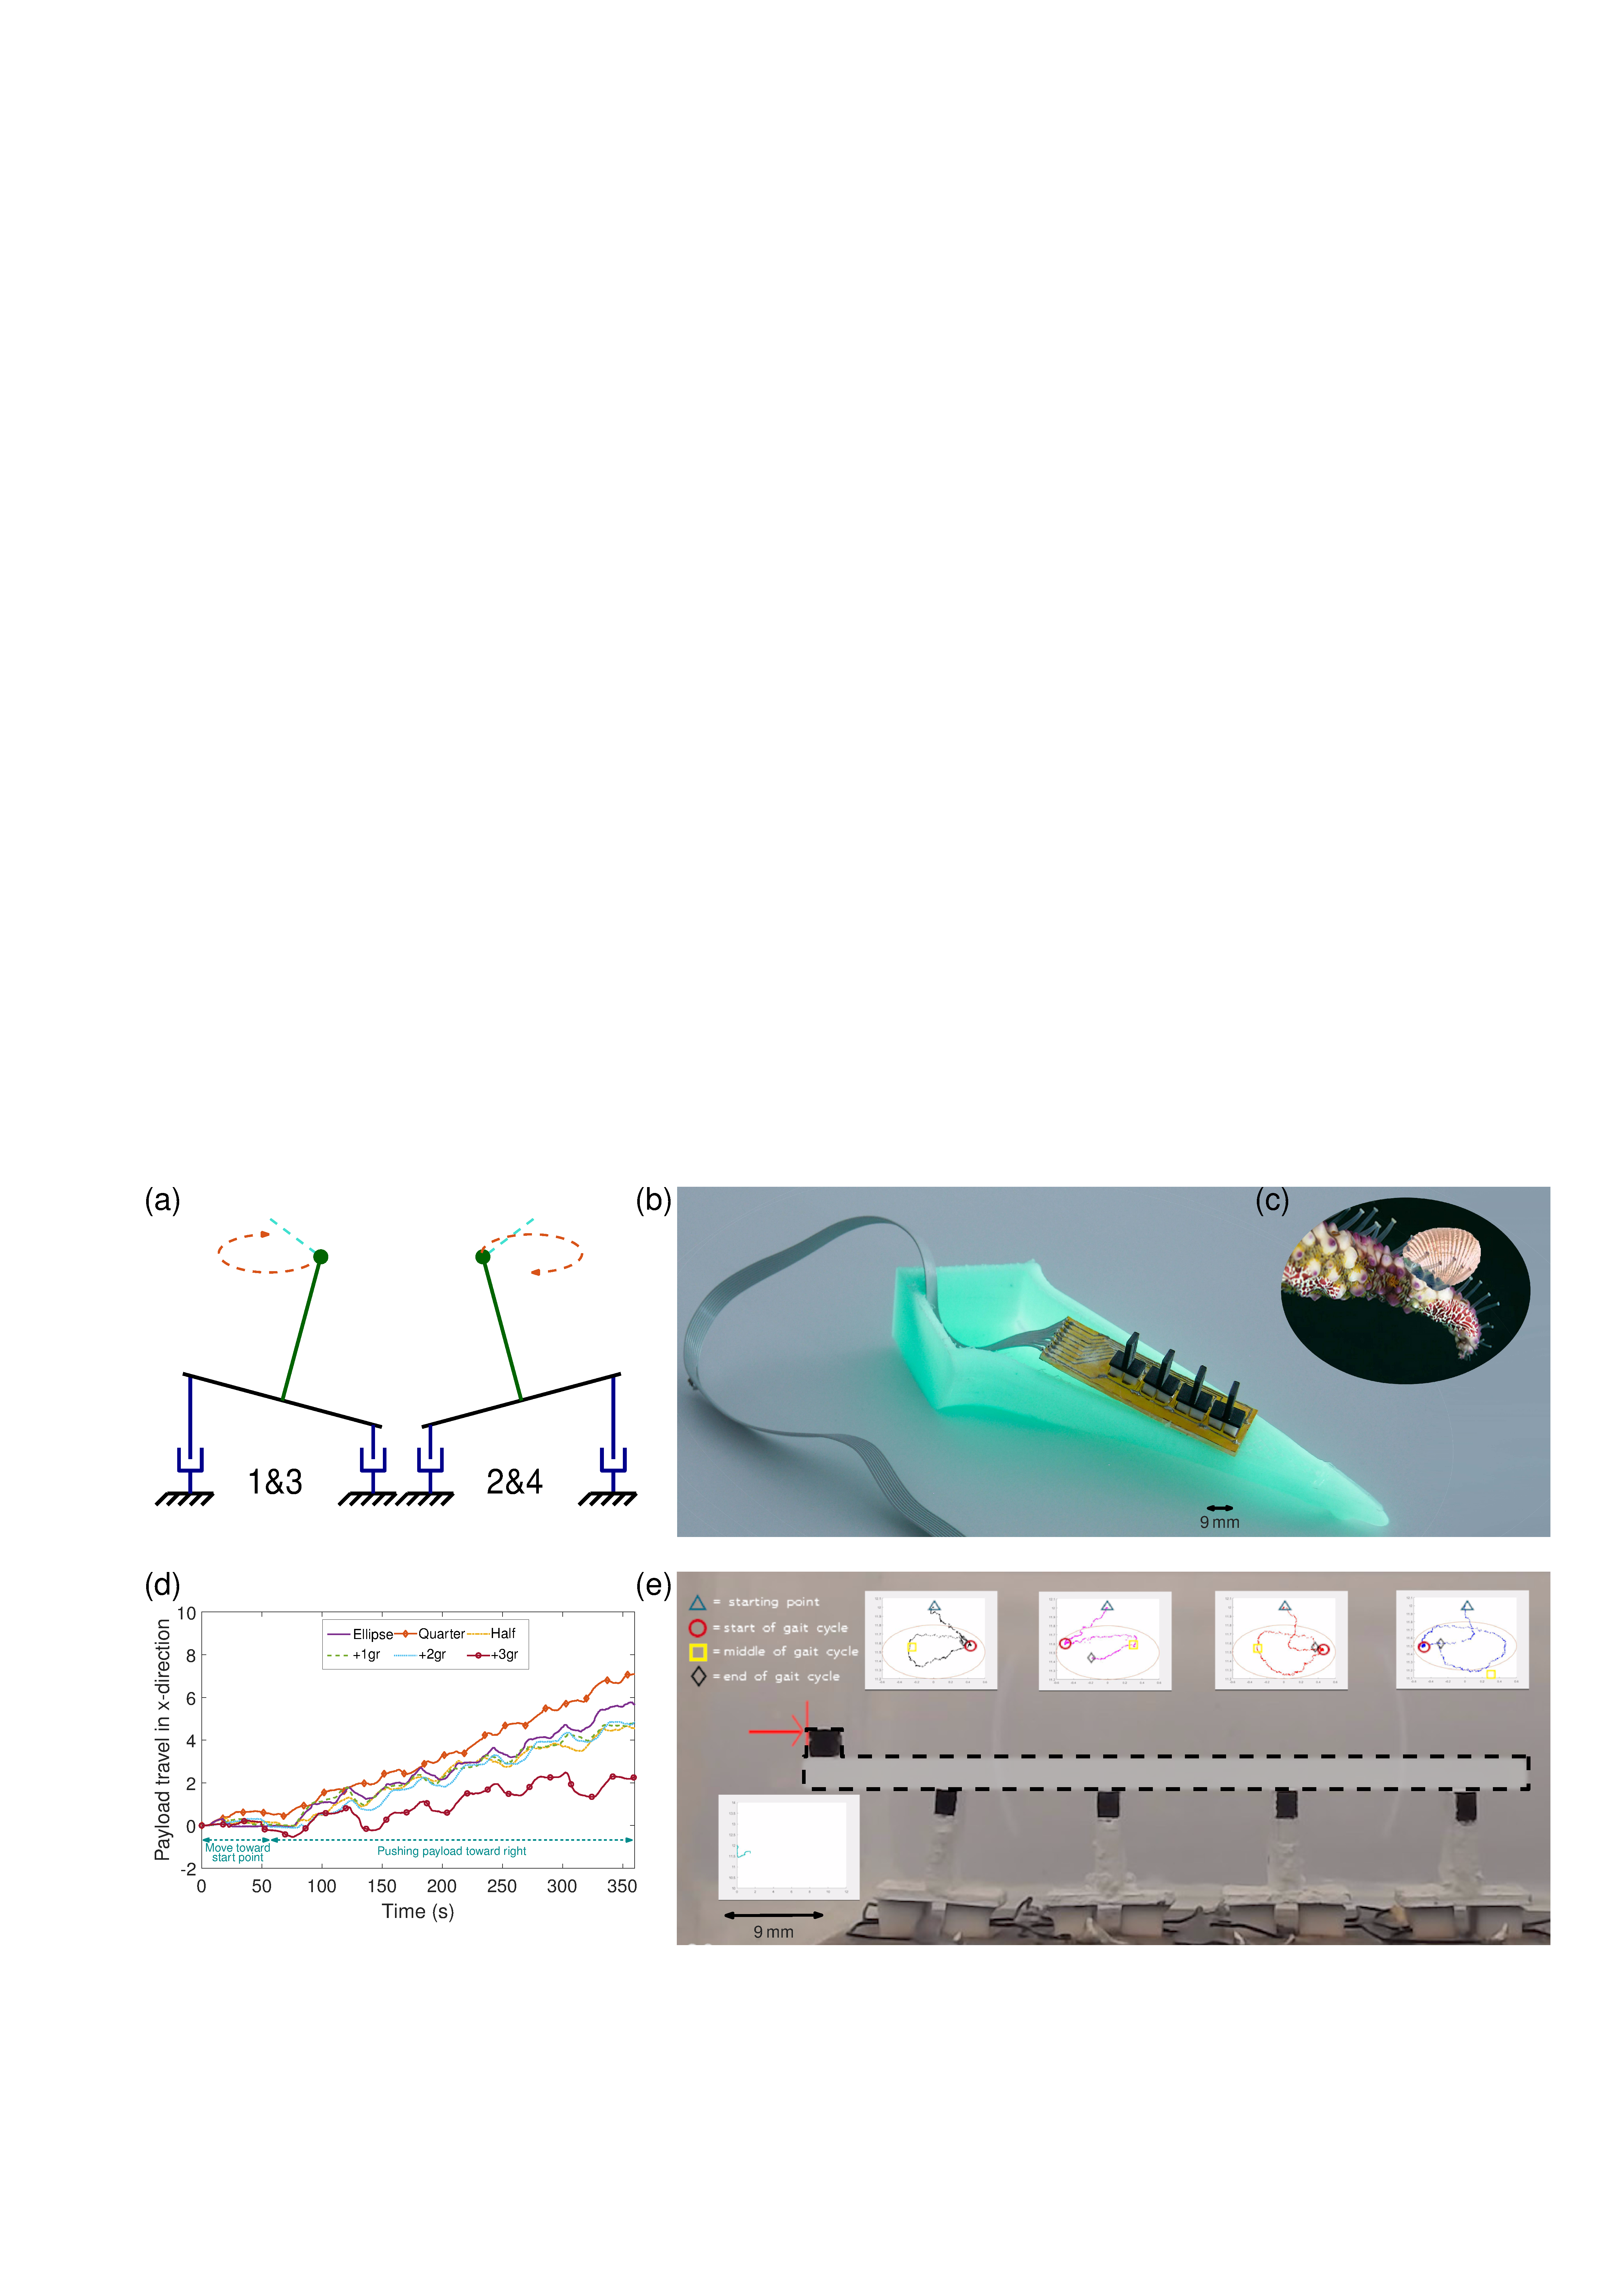
\includegraphics[width=\textwidth]{Starfish_tube_feet_application_8.pdf}}
%\caption[Control of four 9\,mm manipulators in series for payload transport]{Control of four 9\,mm manipulators in series for payload transport, in a manner similar to food transport by starfish tube feet. (a) The manipulators, numbered 1 to 4 from left to right, are commanded to first follow the cyan dashed lines from their initial positions to their starting positions on the reference trajectories, and then follow these  trajectories, shown as red dashed lines. Manipulators 1 and 3 have a phase shift of $180^\circ$ compared to manipulators 2 and 4. (b) Illustration of a starfish-inspired robotic platform with four hydrogel-actuated manipulators. (c) Real starfish transporting a clam on its tube feet. (d) Displacement of the payload as a function of time for different reference trajectories and load weights. (e) Array of four manipulators functioning as described in (a) to transport the payload. Image was taken when the manipulators completed the first gait cycle. The payload is a clear flat acrylic plate with a black square on its left side. The positions of the manipulator tips are marked by triangles at their initial locations, circles at the start of the gait cycle, squares at the middle of the gait cycle, and diamonds at the end of the gait cycle.
%}
    %\label{fig:Control_payload}
%\end{figure*}
%In order to further characterize our system's actuation capabilities, the manipulator's trajectory-tracking performance under load was studied, as shown in Fig.~\ref{fig:Control_outputs}i. Loads (stainless steel nuts) weighing 1\,g, 2\,g, and 3\,g were placed on the 25\,mm extension, as shown in Fig.~\ref{fig:Path}b. The manipulator was commanded to follow the same elliptical trajectory as in the unloaded case. The results show that the addition of a weight of up to 3\,g increases the trajectory tracking NMAE from 8.1$\%$ to 10.2$\%$ (see Table~\ref{table:control}). Despite the increase in error, each actuator is still able to function under a load as large as 12.5 times its own weight (0.12\,g).
%% Tracking the given trajectories requires each SVA to cycle through multiple phases of heating and cooling. As can be observed in Fig.~\ref{fig:Control_outputs}, tracking error is evident for each reference trajectory.The largest tracking error in all cases occurs along a portion of the trajectory in the lower left quadrant of the plots, in which, both SVAs are cooling. Accounting for the different time-constants of the SVAs in heating and cooling states, this transition is not well-characterized in our model obtained by black-box system identification, which results in less accurate trajectory tracking along this portion. We believe, therefore, that the largest difference between our simulated and experimental results can be attributed to the model's inability to characterize the state of SVA heating or cooling. 
%As shown in Table~\ref{table:control}, the experimental NMAE values are higher than the simulation values, but remain below $15$\%.
%
%
%\subsection{Payload transport application} \label{sec:payload}
%Inspired by the way starfish transport food using their tube feet (Figs.~\ref{fig:Control_payload}b and~\ref{fig:Control_payload}c)~\cite{Kerkut1953,Pentreath1970}, we configured an array of four 9\,mm manipulators, as shown in Fig.~\ref{fig:Control_payload}e, and applied the proposed $H_\infty$-optimal controller in~\eqref{eq:Hinf-ctl} and Fig.~\ref{fig:control_block}b to each manipulator in order to transport a payload across their tips. The payload being transported is a clear acrylic plate. The manipulators are commanded to track reference trajectories as depicted in Fig.~\ref{fig:Control_payload}a, with phase shifts between adjacent manipulators. The payload moves to the right as the manipulators complete repeated cycles of the reference trajectories (``gait cycles''), as shown in Figs.~\ref{fig:Control_payload}d and~\ref{fig:Control_payload}e. The data from Fig.~\ref{fig:Control_payload}d on the duration of one gait cycle and the payload displacement in each tested scenario including the ones with extra added loads on the payload are reported in Table~\ref{table:table_Payload displacement}. A video of the payload transport is attached as supplementary material. The payload's position is recorded but not controlled in this exemplar application, since our goal in this chapter was to demonstrate a use-case for trajectory tracking control. However, many other platforms and applications are possible, including bio-inspired ones~\cite{Doroudchi2020}. Through this example, we have demonstrated how trajectory tracking control of systems with soft actuators, when applied to even simple platforms such as this 2-DOF manipulator, may be used to complete complex tasks such as object transport when used in parallel. This type of design can be used to simplify and decouple the control structures in future applications to reduce computational expense.
%
%\begin{table}[t]
%\centering
%\caption{Payload displacement $\Delta X$ with different reference trajectories for the manipulators.}
%\label{table:table_Payload displacement}
%\begin{tabular}{c c c c}
%
%% & & \\ 
%\hline
%Reference & Payload weight & Time for one & $\Delta X$ after five \\
%trajectory & + load (g) & gait cycle (s) & gait cycles (mm)\\
%\hline
%Ellipse         & 2.7   & 60  & 5.66\\
%Half-ellipse    & 2.7   & 50  & 4.55\\
%Quarter-ellipse & 2.7   & 40  & 7.10\\
%Ellipse         & 2.7+1 & 60  & 4.75\\
%Ellipse         & 2.7+2 & 60  & 4.84\\
%Ellipse         & 2.7+3 & 60  & 2.30\\
%% Open-loop  & 2.7~g & N/A & 2.04~mm\\
%\hline
%\end{tabular}
%\end{table}

%------------------------------------------------------
\subsection{prove that the ${H_{\infty}}$ gain is bounded}
%\appendix
We can prove that the ${H_{\infty}}$ gain is bounded using the bounded-real lemma~\cite{Boyd1994} below. 
% \vspace{1mm}

\textbf{Lemma}: \textit{Suppose that}
\begin{equation*}
\vect{G}(s)=\begin{bmatrix}
\begin{array}{c | c}
\vect{A}  &  \vect{B} \\
\hline
\vect{C}  & \vect{D}
\end{array}  
\end{bmatrix}.
\end{equation*}

\textit{Then, the following statements are equivalent:} 

1.~~$\norm{\vect{G}(s)}_{H_{\infty}}$ $\leq$ $\gamma$ \vspace{1mm}
    
2.~~There exists a $\vect{P} > 0$ such that 

    \begin{equation*}
		\begin{bmatrix}
		\vect{A}^T\vect{P}+\vect{PA} &  \vect{PB} \\
		\vect{B}^T\vect{P}    & -\gamma \vect{I} \\
		\end{bmatrix}+\dfrac{1}{\gamma}	\begin{bmatrix}
		\vect{C}^T\\
		\vect{D}^T\\
		\end{bmatrix}\begin{bmatrix}
		\vect{C} & \vect{D}\\
		\end{bmatrix} < 0
        %\vspace{-2mm}
		\label{eq-LMI}
		\end{equation*}

The proof that statement 1 implies 2 requires the Hamiltonian, and the proof that statement 2 implies 1 uses the global stability conditions of the Lyapunov function~\cite{Boyd1994}.
\section{Conclusion}

In this chapter, we addressed a trajectory-tracking problem for a millimeter-scale 2-DOF manipulator with soft hydrogel-based actuators. We defined a linear state-space model of the manipulator and fit the matrices of this model using input-output measurement black-box identification. This state-space representation enables the implementation of a range of controllers on the manipulator; in this chapter, the performance of an observer-based controller was compared in simulation to that of an $H_{\infty}$-optimal controller in an output-feedback framework with and without noise and disturbance. We showed experimentally that different versions of the manipulator are able to track various reference trajectories, even under load, using the $H_{\infty}$-optimal controller.

Our ability to coordinate independently controllable soft actuators with complex internal dynamics in a robotic system demonstrates progress in the real-time, closed-loop control of mechanisms with this type of actuator. We expect that researchers will be able to adapt this approach across similar stimuli-responsive materials as they are developed and optimized. This will also permit SVAs, manufactured from a variety of materials, to be used for controlled grasping, manipulation, and locomotion tasks across a variety of new soft robotic platforms, such as octopus-inspired continuum robots~\cite{Doroudchi2020}. Our approach can be used to design and implement decentralized controllers on segmented mechanisms with distributed hydrogel actuators, as discussed in our related work~\cite{Doroudchi2020,Doroudchi2019}.

In future work, we plan to improve the speed of the image processing algorithms for tracking the manipulator, and ultimately eliminate the use of the camera for position tracking and instead implement this control scheme using embedded sensor feedback.  This will enable the application of machine learning techniques to optimize control performance.

